\ifdefined\beamerclass
\else
    \def\beamerclass{beamer}
\fi
\documentclass[\beamerclass]{beamer}

\usepackage{pgfpages}
\mode<handout>{
  % \setbeamercolor{background canvas}{bg=black!20}
  \pgfpagesuselayout{2 on 1}[a4paper,border shrink=5mm]
}

\mode<presentation>
{\usetheme{default}
 \usecolortheme{default}
 \usefonttheme{default}
 \setbeamertemplate{navigation symbols}{}
 \setbeamertemplate{footline}[frame number]
% \setbeamertemplate{caption}[numbered]
 }
\usepackage[english]{babel}
\usepackage{algorithm}
\usepackage[noend]{algpseudocode}
\usepackage[utf8x]{inputenc}
\usepackage{graphicx}
\usepackage{hyperref}
%\graphicspath{{./images/}}
\usepackage{tikz}
\usetikzlibrary{shapes.geometric, arrows,chains}
\usepackage{booktabs,makecell,multirow,tabularx}
\usepackage{verbatim}
\renewcommand{\arraystretch}{1.2}
\renewcommand\theadfont{\normalfont\bfseries}
\usepackage{array}
\usepackage{listings}
\lstset{language=Java, showstringspaces=false}
\usepackage[normalem]{ulem}
\usepackage{bm}
\def\layersep{2.5cm}

\usepackage{xcolor}
%\usepackage{subfig}
\setbeamertemplate{caption}{\insertcaption}
\usepackage[caption=false]{subfig}
\usepackage{hyperref}
\usepackage{verbatim}
%\setbeamertemplate{caption}[numbered]%\numberwithin{figure}{section}
% Define block styles
\tikzstyle{decision} = [diamond, draw, fill=blue!20, 
    text width=4.5em, text badly centered, node distance=3cm, inner sep=0pt]
\tikzstyle{block} = [rectangle, draw, fill=blue!20, 
    text width=3em, text centered, rounded corners, minimum height=3em]
\tikzstyle{line} = [draw, -latex']
\tikzstyle{cloud} = [draw, ellipse, fill=red!20, node distance=3cm,
    minimum height=2em]
\tikzset{
  startstop/.style={
    rectangle, 
    rounded corners,
    minimum width=3cm, 
    minimum height=1cm,
    align=center, 
    draw=black, 
    fill=red!30
    },
  process/.style={
    rectangle, 
    minimum width=3cm, 
    minimum height=1cm, 
    align=center, 
    draw=black, 
    fill=blue!30
    },
  decision/.style={
    rectangle, 
    minimum width=3cm, 
    minimum height=1cm, align=center, 
    draw=black, 
    fill=green!30
    },
  arrow/.style={thick,->,>=stealth},
  dec/.style={
    ellipse, 
    align=center, 
    draw=black, 
    fill=green!30
    },
}
\tikzstyle{arrow} = [thick,->,>=stealth]

\tikzset{onslide/.code args={<#1>#2}{%
  \only<#1>{\pgfkeysalso{#2}} % \pgfkeysalso doesn't change the path
}}

\makeatletter
\newenvironment<>{btHighlight}[1][]
{\begin{onlyenv}#2\begingroup\tikzset{bt@Highlight@par/.style={#1}}\begin{lrbox}{\@tempboxa}}
{\end{lrbox}\bt@HL@box[bt@Highlight@par]{\@tempboxa}\endgroup\end{onlyenv}}

\newcommand<>\btHL[1][]{%
  \only#2{\begin{btHighlight}[#1]\bgroup\aftergroup\bt@HL@endenv}%
}
\def\bt@HL@endenv{%
  \end{btHighlight}%   
  \egroup
}
\newcommand{\bt@HL@box}[2][]{%
  \tikz[#1]{%
    \pgfpathrectangle{\pgfpoint{1pt}{0pt}}{\pgfpoint{\wd #2}{\ht #2}}%
    \pgfusepath{use as bounding box}%
    \node[anchor=base west, fill=orange!30,outer sep=0pt,inner xsep=1pt, inner ysep=0pt, rounded corners=3pt, minimum height=\ht\strutbox+1pt,#1]{\raisebox{1pt}{\strut}\strut\usebox{#2}};
  }%
}
\makeatother




%%%%%%%%%%%%%%%%%%%%%%%%%%%%%%%%%%%%%%%%%%%%%%
% Formatting for title page
\title[Deep Learning]{Autoencoder Architectures}
\author{Kate Farrahi}
\institute{ECS Southampton}
\date{\today}
%%%%%%%%%%%%%%%%%%%%%%%%%%%%%%%%%%%%%%%%%%%%%%
\begin{document}
\begin{frame}
  \titlepage
\end{frame}
%-------------------------------------------------------------%

%\begin{frame}[fragile]{pause}\frametitle{Vanishing Gradients in RNNs}
%\end{frame}
%-------------------------------------------------------------%
\begin{frame}[fragile]{pause}\frametitle{ Autoencoder}
The aim of an autoencoder is to learn a representation (encoding) for a set of data, typically for dimensionality reduction, by training the network to ignore signal noise. 
\begin{center}
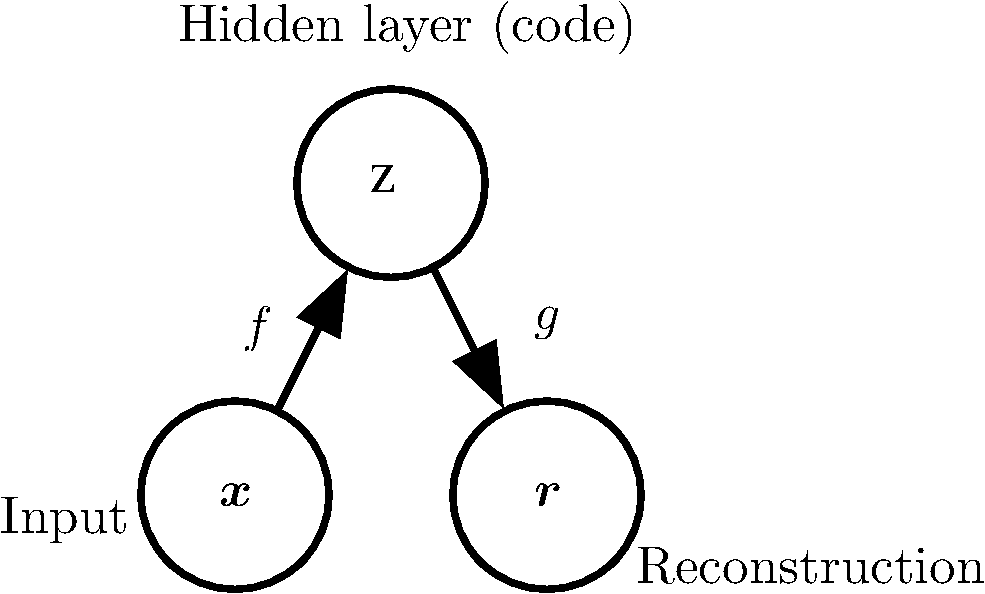
\includegraphics[width=7cm]{AE.pdf} \footnote{Image taken from Deep Learning book by Goodfellow et al.}
\end{center}
\end{frame}
%-------------------------------------------------------------%

\begin{frame}[fragile]{pause}\frametitle{Deep Autoencoder}
\begin{center}
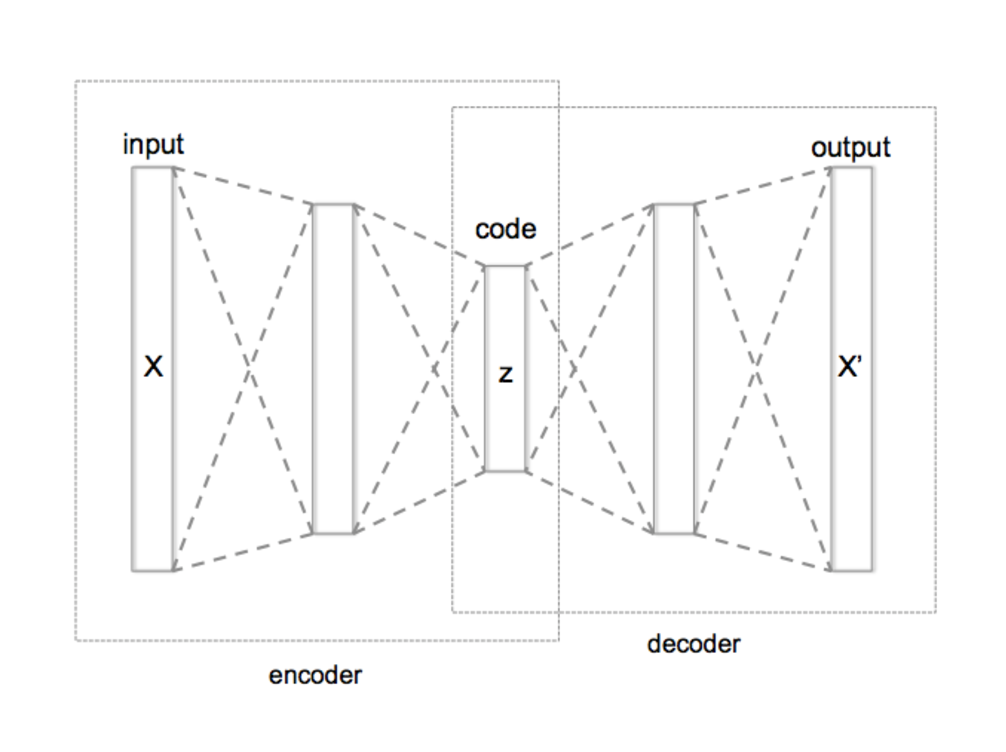
\includegraphics[width=10cm]{DAE.pdf} \footnote{Image taken from wikipedia}
\end{center}
\end{frame}
%-------------------------------------------------------------%

\begin{frame}[fragile]{pause}\frametitle{Denoising Autoencoder}
\begin{itemize}
\item Denoising autoencoders take a partially corrupted input and train to recover the original undistorted input. \pause
\item To train an autoencoder to denoise data, it is necessary to perform a preliminary stochastic mapping to corrupt the data ($x \rightarrow \tilde x$).  \pause
\item A normal autoencoder is used with $\tilde x$ is used as input and $ x$ as output. \pause
\item In a denoising autoencoder, the loss should be computed on $\mathcal{L}(x, \hat x)$ as opposed to $\mathcal{L}(\tilde x, \hat x)$.
\end{itemize}
\end{frame}
%-------------------------------------------------------------%


\begin{frame}[fragile]{pause}\frametitle{Sparse Autoencoder}
\begin{itemize}
\item In a sparse autoencoder, there are more hidden units than inputs, but only a small number of the hidden units are allowed to be active at the same time.
\end{itemize}
\end{frame}
%-------------------------------------------------------------%


\begin{frame}[fragile]{pause}\frametitle{Autoencoder Applications}
\begin{itemize}
\item Any basic AE (or its variant) is used to learn a compact representation of data. \pause
\item You can learn automatic features from data. E.g. HAR with sensor data. \pause
\item Denoising can help generalise over the test set since the data is distorted by adding noise. \pause
\item Pretraining networks by learning your network weights using a stacked AE.
\end{itemize}
\end{frame}
%-------------------------------------------------------------%

\begin{frame}[fragile]\frametitle{Variational Autoencoders (VAEs)}
%\begin{center}
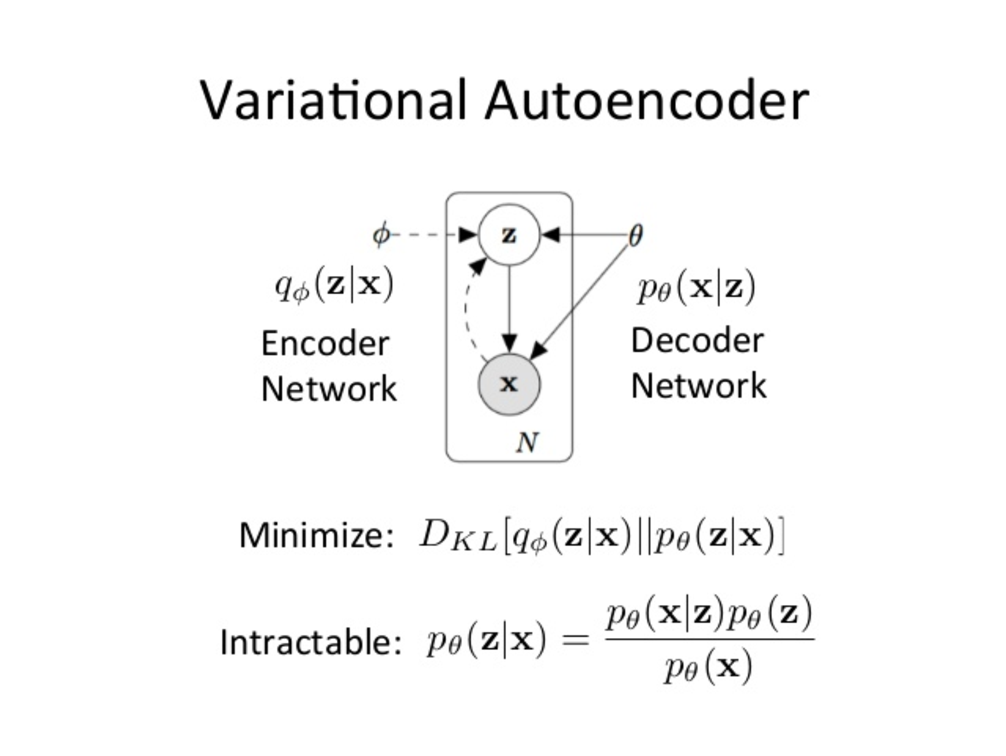
\includegraphics[width=10cm]{VAE.pdf} \footnote{Slide taken from \url{https://www.slideshare.net/ckmarkohchang/variational-autoencoder}}
%\end{center}
\end{frame}
%-------------------------------------------------------------%

\begin{frame}[fragile]{pause}\frametitle{Variational Autoencoder}
\begin{itemize}
\item In VAEs, data is generated by a directed graphical model $p(x|z)$. \pause
\item The encoder is learning an approximation $q_{\phi}(z|x)$ to the posterior distribution $p_{\theta}(x|z)$, where $\phi$ and $\theta$ denote the parameters of the encoder and decoder, respectively. \pause
\item The objective of the VAE has the following form $\mathcal{L} = D_{KL}(q_{\phi}(z|x) || p_{\theta}(z)) - \mathop{\mathbb{E}}_{q_{\phi}}(log  p_{\theta}(x|z))$
\end{itemize}
\end{frame}
%-------------------------------------------------------------%

\end{document}